%\documentclass[preprint]{sigplanconf}
%\documentclass[preprint]{llncs}
\documentclass[a4paper,UKenglish]{lipics-v2016}

\usepackage{microtype}%if unwanted, comment out or use option "draft"
\usepackage[table,xcdraw]{xcolor}
\usepackage{color}
\usepackage{amsmath}
\usepackage{stmaryrd}
\usepackage{graphicx}
\usepackage{amssymb}
\usepackage{fancyvrb}
\usepackage{url}
\usepackage{pstricks,pst-node,pst-tree}
\usepackage{theorem}
\usepackage{syntax}
\usepackage{bbm}
\usepackage{pgf}
\usepackage{multirow}

\usepackage{listings}
\usepackage{verbatim}
\usepackage{graphicx}
\usepackage{wrapfig}

\usepackage[T1]{fontenc}
\usepackage[scaled=0.85]{beramono}
\usepackage{mathpartir}

% "define" code highlights for Java and Scala
\lstdefinelanguage{JavaScala}{
  morekeywords={public,int,interface,implements,default,
    abstract,case,catch,class,def,static,%
    do,else,extends,false,final,finally,%
    for,if,implicit,import,match,mixin,%
    new,null,object,override,package,%
    private,protected,requires,return,sealed,%
    super,this,throw,trait,true,try,%
    type,var,while,yield,with,val},
  otherkeywords={=>,<\%,<:,>:,\#,@},
  sensitive=true,
  morecomment=[l]{//},
  morecomment=[n]{/*}{*/},
  morestring=[b]",
  morestring=[b]',
  morestring=[b]"""
}

\lstdefinelanguage{PlainCode}{}

\lstset{ %
language=JavaScala,                % choose the language of the code
columns=flexible,
lineskip=-1pt,
basicstyle=\ttfamily\small,       % the size of the fonts that are used for the code
numbers=none,                   % where to put the line-numbers
numberstyle=\ttfamily\tiny,      % the size of the fonts that are used for the line-numbers
stepnumber=1,                   % the step between two line-numbers. If it's 1 each line will be numbered
numbersep=5pt,                  % how far the line-numbers are from the code
backgroundcolor=\color{white},  % choose the background color. You must add \usepackage{color}
showspaces=false,               % show spaces adding particular underscores
showstringspaces=false,         % underline spaces within strings
showtabs=false,                 % show tabs within strings adding particular underscores
morekeywords={var, lazy},
%  frame=single,                   % adds a frame around the code
tabsize=2,                  % sets default tabsize to 2 spaces
captionpos=none,                   % sets the caption-position to bottom
breaklines=true,                % sets automatic line breaking
breakatwhitespace=false,        % sets if automatic breaks should only happen at whitespace
title=\lstname,                 % show the filename of files included with \lstinputlisting; also try caption instead of title
escapeinside={(**}{**)},          % if you want to add a comment within your code
keywordstyle=\ttfamily\bfseries,
% commentstyle=\color{Gray},
% stringstyle=\color{Green}
}


%%\usepackage{natbib}
%%\bibpunct();A{},
%%\let\cite=\citep

%include lhs2TeX.fmt
%include lhs2TeX.sty
%include forall.fmt

%\pagestyle{plain}

%{\theorembodyfont{\sffamily} \newtheorem{theorem}{Theorem}}
%{\theorembodyfont{\sffamily} \newtheorem{lemma}{Lemma}}
%\newtheorem{theorem}{Theorem}
%\newtheorem{lemma}{Lemma}
%\newenvironment{proof}{\textbf{Proof:\hspace{4mm}}}{$\Box$}
\newcommand\inlinecode[1]{\lstinline[language=PlainCode]{#1}}
\newcommand{\authornote}[3]{{\color{#2} {\sc #1}: #3}}
\newcommand\bruno[1]{\authornote{bruno}{red}{#1}}
\newcommand\yanlin[1]{\authornote{yanlin}{purple}{#1}}
%\newcommand{\hl}[1]{\textcolor{red}{#1}}
\newcommand\huang[1]{\authornote{huang}{blue}{#1}}
\newcommand\haoyuan[1]{\authornote{haoyuan}{cyan}{#1}}

\newcommand\sem[1]{\llbracket #1 \rrbracket_r}
\newcommand\sems[1]{\llbracket #1 \rrbracket_s}
\newcommand\tsem[1]{\llbracket #1 \rrbracket}
\newcommand{\rbm}[1]{\raisebox{-2.0ex}[0.5ex]{#1}}
\newcommand\nat[0]{\mathbb{N}}
\newcommand\unit[0]{\mathbbm{1}}

\newcommand\mixin{\textbf{@Mixin} }
\newcommand\name{\textbf{Parser}\xspace}
\usepackage{xspace}
\renewcommand{\paragraph}[1]{\vspace{2pt}\noindent {\bf #1}}

% Author macros::begin %%%%%%%%%%%%%%%%%%%%%%%%%%%%%%%%%%%%%%%%%%%%%%%%
\title{Type-Safe Modular Parsing}
\titlerunning{Type-Safe Modular Parsing}
\author[1]{}

%% Please provide for each author the \author and \affil macro, even when authors have the same affiliation, i.e. for each author there needs to be the  \author and \affil macros
%\author[1]{John Q. Open}
%\author[2]{Joan R. Access}
%\affil[1]{Dummy University Computing Laboratory, Address/City, Country\\
%  \texttt{open@dummyuniversity.org}}
%\affil[2]{Department of Informatics, Dummy College, Address/City, Country\\
 % \texttt{access@dummycollege.org}}
%\authorrunning{J.\,Q. Open and J.\,R. Access} %mandatory. First: Use abbreviated first/middle names. Second (only in severe cases): Use first author plus 'et. al.'

%\Copyright{John Q. Open and Joan R. Access}%mandatory, please use full first names. LIPIcs license is "CC-BY";  http://creativecommons.org/licenses/by/3.0/

%\subjclass{Dummy classification -- please refer to \url{http://www.acm.org/about/class/ccs98-html}}% mandatory: Please choose ACM 1998 classifications from http://www.acm.org/about/class/ccs98-html . E.g., cite as "F.1.1 Models of Computation".
%\keywords{Dummy keyword -- please provide 1--5 keywords}% mandatory: Please provide 1-5 keywords
% Author macros::end %%%%%%%%%%%%%%%%%%%%%%%%%%%%%%%%%%%%%%%%%%%%%%%%%

%Editor-only macros:: begin (do not touch as
%author)%%%%%%%%%%%%%%%%%%%%%%%%%%%%%%%%%%
\begin{comment}
\EventEditors{John Q. Open and Joan R. Acces}
\EventNoEds{2}
\EventLongTitle{42nd Conference on Very Important Topics (CVIT 2016)}
\EventShortTitle{CVIT 2016}
\EventAcronym{CVIT}
\EventYear{2016}
\EventDate{December 24--27, 2016}
\EventLocation{Little Whinging, United Kingdom}
\EventLogo{}
\SeriesVolume{42}
\ArticleNo{23}
\end{comment}
% Editor-only macros::end %%%%%%%%%%%%%%%%%%%%%%%%%%%%%%%%%%%%%%%%%%%%%%%

%%%%%%%%%%%%%%%%%%%%%%%%%%%%%%%%%%%%%%%%%%%%%%%%%%%%%%%%%%%%%%%%%%%%%%%%%%%%%%%%
\begin{document}
\maketitle

\begin{abstract}

  Over the years a lot of effort has been put on solving challenging
  extensibility problems, while retaining important software
  engineering properties such as modular type-safety and
  separate compilation. Most previous work focused on
  operations that traverse and process extensible Abstract Syntax Tree
  (AST) structures. However, there is almost no work on operations that
  \emph{build} such extensible ASTs, including \emph{parsing}.

  This paper investigates solutions for the problem of \emph{modular
    parsing}. We focus on \emph{semantic} modularity and not just
  \emph{syntactic} modularity. That is, the solutions should not only
  allow complete parsers to be built out of modular parsing
  components, but also enable the parsing components to be
  \emph{modularly type-checked} and \emph{separately compiled}. We
  present a technique based on parsing combinators that enables modular
  parsing. Interestingly, the modularity requirements for modular
  parsing rule out several existing parsing combinator approaches,
  which rely on some non-modular techniques. We show that Packrat
  parsing techniques, provide solutions for such modularity problems,
  and enable reasonable performance in a modular setting.
  Extensibility is achieved using \emph{multiple inheritance} and
  \emph{Object Algebras}.  To evaluate
  the approach we conduct a case study based on the ``Types and
  Programming Languages'' interpreters. The case study shows the
  effectiveness at reusing parsing code from existing interpreters,
  and the total parsing code is 69\% shorter than an existing code
  base using non-modular parsing code.

\end{abstract}

%if False

%\category{D.3.2}{Programming Languages}
%                {Language Classifications}
%                [Functional Languages]
%\category{F.3.3}{Logics and Meanings of Programs}
%                {Studies of Program Constructs}
%                []

%\terms
%Languages
%
%\keywords
%Mixins, explicit effects, monads, aspect-oriented programming, parametricity,
%interference

%endif

%===============================================================================

\section{Introduction}\label{sec:introduction}
 
The quest for improved modularity, variability and extensibility of
programs has been going on since the early days of Software
Engineering~\cite{McIlroy68}. Modern Programming Languages (PLs) enable a certain
degree of modularity, but they have limitations as illustrated by
well-known problems such as the Expression Problem~\cite{wadler1998expression}. The
Expression Problem refers to the difficulty of writing data
abstractions that can be easily extended with both new operations and
new data variants. Traditionally the kinds of data abstraction found
in functional languages can be extended with new operations, but
adding new data variants is difficult. The traditional object-oriented
approach to data abstraction facilitates adding new data variants
(classes), while adding new operations is more difficult.

\begin{comment}
A reason why a solution to the Expression Problem is important in
practice is that it is necessary for the development of
\emph{Software-Product Lines} (SPLs)~\cite{}. A software-product line
is a reusable set of components, which can be combined in multiple ways
to obtain different programs. Programming languages offer a concrete
example for SPLs. A SPL for programming languages would allow us to
model various typical operations of programming languages (such as
evaluation, compilation, or parsing) for various different language
constructs (such as binding, arithmetic, conditional or loops)
independently and separately. For example, evaluation components could be defined
independently for binding and arithmetic constructs. If the language
to be implemented is the pure lambda calculus, only evaluation of
binding constructs is necessary. However, more realistic programming
languages will include arithmetic constructs, and will require 
evaluation for such constructs as well. In this case 
both the component for evaluation of binders and arithmetic 
expressions can be combined to implement the desired functionality.
\end{comment}

\begin{comment}
Most programming languages share alot of features in
common. 

For example, most languages have language constructs for:
binding (such as variables, functions, and function applications);
basic arithmetic operations; basic logic and conditional operations;
loops; as well as various other features. For each language construct,
various operations (such as evaluation, compilation, or parsing) need
to be implemented. It is reasonable to wonder whether we can simply
implement those features independently of a particular implementation
of a programming language. Evaluation could be defined independently 
for binding and arithmetic constructs. If the language to be
implemented is the pure lambda calculus, only evaluation of binding 
constructs is necessary. Thus only the component that implements 
evaluation for binding needs to be used in such an implementation.
However, more realistic programming languages 
will include arithmetic constructs, and will require an evaluation
function for those. 


Then it would be possible to \emph{reuse}
some of those features in \emph{multiple} different implementations of
programming languages. Essentially, this would enable a SPL for
programming languages, where all

A solution to the Expression Problem could ena



A concrete 
example that illustrates this issue is 
\end{comment}

To address the modularity limitations of Programming Languages several
different approaches have been proposed in the past. Existing
approaches can be broadly divided into two categories:
\emph{syntactic} or \emph{semantic} modularization
techniques. Syntactic modularization techniques are quite popular in
practice, due to their simplicity of implementation and use. 
Examples include many tools for developing Software-Product
Lines~\cite{}, some Language Workbenches~\cite{}, or extensible parser
generators~\cite{}.  Most syntactic approaches employ textual
composition techniques such as \emph{superimposition}~\cite{} to
enable the development modular program features. Such textual
composition techniques collect the code for multiple features and
merge it together when a concrete combination of features is needed
for a particular program. As Kastner et. al~\cite{Kastner11road} note, the typical
drawback of such techniques is that
``\emph{most feature-oriented implementation mechanisms lack proper
  interfaces and support neither modular type checking nor separate
  compilation}''. 

Syntactic modularization techniques have also been applied to the
problem of \emph{extensible parsing}. There are several approaches
that enable the development of \emph{syntactically} modular parsers or
grammars. Many parser
generators~\cite{antlr1995,Grimm2006,Gouseti2014,Warth2016} support
modular grammars. For instance, \textit{Rats!}~\cite{Grimm2006} has
its own module system for the collection of grammars.  Extensible
compilers like JastAdd~\cite{Ekman2007} and
Polyglot~\cite{Nystrom2003} also support extensible parsing, but this
is mostly done ultimately resorting to standard (non-modular) parser
generators. Various techniques supporting languages that can extend
their own syntax, such as SugarJ~\cite{Erdweg2011}, also offer a form
of extensible parsing. However these syntactic approaches do not
support separate compilation and/or modular type-checking of parsing
code either.

Semantic modularization techniques go one step further in terms of modularity,
and also enable components or features to be modularly type-checked
and separately compiled. Modular type-checking and separate
compilation are desirable properties to have from a software
engineering point-of-view. Modular type-checking can report errors 
earlier and in terms of the modular code programmers have written 
in the first place. Separate compilation avoids global compilation
steps, which can be very costly. Furthermore semantic modularization 
enables the composition of compiled binaries as well as ensuring the 
type-safety of the code composed of multiple components. Examples of semantic modularization techniques 
include various approaches to \emph{family polymorphism}~\cite{ernst01FP},
\emph{virtual classes}~\cite{Ernst:2006}, as 
well as several other techniques for solving the Expression
Problem~\cite{Oliveira:2012}\bruno{more here; yanlin; Torgersen; Odersky...}. 

Semantic modularization techniques are less widely used in practice 
than syntactic techniques. This is partly due to the need
for more sophisticated type systems, which are not available in mainstream 
languages and may require more knowledge from users. However, recently 
several lightweight modularization techniques have been shown to work 
in mainstream programming languages like Java or Scala. Object
Algebras~\cite{Oliveira:2012} are one such technique, which works in
Java-like languages and uses simple generics only. So far research on semantic
modularization techniques have focused on operations that \emph{traverse} or 
or \emph{process} extensible datastructures, such as ASTs. Indeed 
many documented applications of semantic modularization techniques
focus on modularizing various aspects of PL implementations.
However, as far as we know there is little work on operations that build/produce ASTs. 
In particular the problem of how to modularize parsing has not been studied in
semantic modularization approaches. This is a shame because parsing
is a fundamental part of PL implementations, and it ought to be
modularized as well.

%\paragraph{Modular and Extensible Parsing}

This paper investigates presents a technique for doing semantically
modular parsing.  That is, our approach not only allows complete
parsers to be built out of modular parsing components, but also enables
those parsing components to be \emph{modularly type-checked} and
\emph{separately compiled}. In developing our techniques we encontered 
two different classes of challenges:

\begin{itemize}

\item {\bf Algorithmic challenges:} A first challenge was todo with
  the parsing algorithms themselves. Since many parsing formalisms
  were not designed with extensibility in mind, some of the employed 
  techniques were non-modular, or performed poorly in a modular setting. 

\item {\bf Typing and Reusability Challenges:} The second class of
  challenges were problems related to modularity, reusability and
  typing.

\end{itemize}

\name is built on top of a Packrat parsing
library, but adds new parsing combinators to enable modular
parsing. The new parsing combinators employ \emph{delegation-based}
techniques and \emph{Object Algebras} to support extensibility. The
choice of Packrat parsing over other parsing techniques turns out to
be important for achieving performance in a modular
setting. \bruno{left recursion, and backtracking removal.}


  By analising the \emph{full} grammar it is possible to remove
  backtracking, which would otherwise increase parsing times. Many
  parsing combinator libraries routinely use backtracting elimination
  to achieve performance. However, in a modular setting this technique
  cannot be used, because the full grammar is not known. Thus we have
  to be very conservative at eliminating backtracting. Unfortunatelly,
  this has a severe impact on performance.

  To evaluate \name we conduct a case study based on the ``Types and
  Programming Languages'' (TAPL) interpreters.  The case study shows
  that \name is effective at reusing parsing code from existing
  interpreters, and the total parsing code is 60\% shorter than the
  non-modular parsing code.\bruno{comment on the efficiency}

In summary our contributions are:

\begin{itemize}

\item {\name:} A parser combinator library that allows the development 
of modular parser. The library uses \emph{delegation} and
\emph{Object-Algebras} to achieve modularity and extensibility.

\item {{\bf A Parsing Technique for OO ASTs:}} A simplified version of
  our technique also enables parsing OO-style ASTs, where new language
  constructs can be easily added.

\item {{\bf Limitations of existing Parser Combinator Techniques:}}
\bruno{Improve and write something here.}

\item {{\bf TAPL case study:}} We conduct a case study with 18 interpreters
  from the TAPL book. The case study show the effectiveness of modular 
  parsing in terms of reuse.

\end{itemize}


\haoyuan{I suggest this part to be moved to Introduction, and only discuss why Packrat is selected among
different parser combinators in Overview.}

\begin{comment}
Although there are many parsing techniques, not all of them are
suitable for type-safe modular parsing. In particular there are many
techniques which fail to provide modular type-checking and separate
compilation. Moreover, even if modular type-checking and separate
compilation are supported, efficiency is another
concern. A parsing technique should have low overhead when applied
in a modular setting. In the remaider of this section, we eliminate
various techniques that fail to satisfy our requirements, and argue
that that Packrat parsing~\cite{Ford2002} is a suitable candidate for
type-safe modular parsing.

\paragraph{Parser Generators} The most widely use tools for parsing
are parser generators. Parser generators help users generate parsers automatically or
semi-automatically from a given grammar. There is no restriction on
the algorithm, while most of them adopts table-based LL~\cite{lewis1968syntax} and LR~\cite{knuth1965translation} parsing
algorithms.
Although efficient, the main drawback of parser generators is that they do not support
modular type-checking and separate compilation.

Modular parsing based on parser generators is supported by many libraries~\cite{antlr1995,Grimm2006,Gouseti2014,Warth2016}. Users can separate the syntax definition and related parsing code into reusable components. Then the corresponding parsers are built by their library utilities. For example, NOA~\cite{Gouseti2014} uses Java annotation processing to collect grammar information, and then generates ANTLR4 parsers. However, such generation procedure requires a whole compilation after the collection of all grammar pieces. Once the grammar changed, even slightly, grammar information must be re-collected and the parser must be re-generated. Hence those libraries only have syntactic modularity.

Generating parsers often requires full information of grammars, thus semantic modularity is difficult to achieve in this way.

\paragraph{Parser Combinators}
Comparing with the parser generators, a \textit{parser combinator}~\cite{burge1975,Wadler1985}
takes several parsers and produce a new parser as its output. Parser combinators are
popular in functional programming, where the parsers are represented
by functions and parser combinators are higher-order functions accepts
them.

At a first look, parser combinators are very suitable for our purpose, because of two
reasons. Firstly, they are naturally modular. The manner of using them
is to write small parsers and use combinators to composed them
together. The construction procedure is explicit and fully controlled
by the programmer. Secondly, each parser combinator is represented by
a piece of code, and also are the parsers it takes. Thus in a
statically typed programming language they can be statically
type-checked.
\end{comment}

\section{Packrat Parsing for Modularity}\label{sec:packrat}

This section discusses the algorithmic challenges introduced by
modular parsing and argues that Packrat parser combinators~\cite{Ford2002}
are suitable to address them. The algorithmic challenges
are important because they rule out various common techniques
used by non-modular code using parser combinators.
To avoid pitfalls related to those algorithmic challenges,
we propose the following methodology:

\begin{itemize}[leftmargin=*]

\item \textbf{Modular parsers should support left-recursion.}

\item \textbf{Modular parsers should use a longest match composition operator.}

\end{itemize}

Moreover, the underlying parsing formalism should make \emph{backtracking
cheap}, due to its pervasiveness in modular parsing.
Although we chose Packrat parsing, any other parsing formalism that provides similar
features should be ok.

\subsection{Algorithmic Challenges of Modularity}\label{subsec:challenges}
For the goal of modular parsing, parser combinators seem suitable because they are
naturally modular for parser composition, but also they ensure type safety.
Unfortunately many parser combinators have important limitations.
In particular, several parser combinators including the famous Parsec~\cite{Leijen2001} library, require
programmers to manually do \textit{left-recursion elimination}, \textit{longest match composition}, and
require significant amounts of \textit{backtracking}. All of those are
problematic in a modular setting.

\paragraph{Left-Recursion Elimination} The top-down, recursive descent parsing strategy adopted by those parser combinator libraries cannot support left-recursive grammars directly. For instance, we start with a simple arithmetic language containing only integers and subtractions. The
grammar with concrete syntax and part of the parsing code in Parsec are presented below:

\begin{minipage}{12em}
\setlength{\grammarindent}{4em}
\begin{grammar}
<expr> ::= <int> \alt <expr> `-' <int>
\end{grammar}
\end{minipage}
\begin{minipage}{15em}
\begin{lstlisting}[language=PlainCode]
parseExpr =
  parseSub <|> parseInt
parseSub = do
  e <- parseExpr ...
\end{lstlisting}
\end{minipage}
Such a left-recursive implementation will cause an infinite loop, since \inlinecode{parseExpr} and \inlinecode{parseSub} call each other and never stop.
A common solution is to rewrite the grammar into an equivalent but non-left-recursive one, called left-recursion elimination:

\vspace{0.4\baselineskip}
\begin{minipage}{15em}
\setlength{\grammarindent}{5em}
\begin{grammar}
<expr> ::= <int> <expr'>

<expr'> ::= <empty> \alt `-' <int> <expr'>
\end{grammar}
\end{minipage}
\vspace{0.4\baselineskip}

\noindent After left-recursion elimination, the structure of grammar is changed,
as well as its corresponding parser. In a modular setting, it is
possible but unnecessarily complicated to analyse the grammar and
rewrite it when doing extensions. Anticipating that every non-terminal
has left-recursive rules is helpful for extensibility but overkill,
since it is inconvenient and introduces extra complexity for
representation of grammars and implementation of parsers.

Another issue of left-recursion elimination is that it requires extra
bookkeeping work to retain the original semantics. For example, the
expression $1-2-3$ is parsed as $(1-2)-3$ in the left-recursive
grammar, but after rewrite the information of left-associativity is lost. The parse tree
must be transformed to recover the correct syntactic structure.

\paragraph{Longest Match Composition} Another problematic issue
in parser combinator libraries is the need for manually prioritizing/ordering
alternatives in a grammar.
Consider the grammar:
\setlength{\grammarindent}{5em}
\begin{grammar}
<expr> ::= <int> \alt <int> `+' <expr>
\end{grammar}

In Parsec, for instance, the parser \inlinecode{"parseInt <|> parseAdd"} will only parse the input \inlinecode{"1 + 2"} to \inlinecode{"1"}, as \inlinecode{parseInt} successfully parses \inlinecode{"1"}
and terminates parsing.

Traditional alternative composition will only find the first parser that succeeds on a prefix of the input,
even if subsequent parsers may parse the whole input. In contrast to the previous parser, \inlinecode{"parseAdd <|> parseInt"} works as expected with because the two cases are swapped.
In this case, reordering the alternatives ensures that
the \emph{longest match} is picked among the possible results. However, manual reordering for the longest match is inconvenient, and worst still, it is essentially non-modular. When the grammar is extended with new rules, programmers should \emph{manually} adjust
the order of parsers, by rewriting previously written code.

\paragraph{Backtracking} The need for backtracking can also be problematic
in a modular setting. Consider a grammar that includes \inlinecode{"import..from"}, 
and is extended with an \inlinecode{"import..as"} case:

\setlength{\grammarindent}{5em}
\begin{grammar}
<stmt> ::= `import' <ident> `from' <ident>
    \alt ...
    \alt `import' <ident> `as' <ident>
\end{grammar}
Since the two cases share a common prefix, when the former fails, we must backtrack to the beginning.
For example, the choice combinator in Parsec only tries the second alternative if the first fails
without any token consumption. We have to use \inlinecode{try} for explicit backtracking.

\begin{lstlisting}[language=PlainCode]
oldParser = parseImpFrom <|> ...
newParser = try parseImpFrom <|> ... <|> parseImpAs
\end{lstlisting}

Similarly, this violates a modular setting because it also requires a global view of the full grammar.
Hence the worst case where all alternatives may share common prefixes with future cases
should always be antecipated. Therefore we need to backtrack for all the branches. To avoid failures in the future, we have to add \inlinecode{try} everywhere. However this results in the worst-case exponential time
complexity.

\subsection{Packrat Parsing}\label{subsec:packratparsing}
Fortunately, some more advanced parsing techniques such as Packrat
parsing~\cite{Ford2002} have been developed to address limitations of
simple parser combinators. Packrat parsing uses memoization to record
the result of applying each parser at each position of the input, so
that repeated computation is eliminated. Moreover, it supports both direct left-recursion
and (in theory) indirect left-recursion~\cite{warth2008}.
All of these properties are very suitable for modularity, thus we decided to use Packrat parsers as the underlying parsing technique for modular parsing.
\begin{comment}
It is worth mentioning that the choice of parser combinators will not
affect the other parts of our library. One can choose other parser
combinators like Parsec, in cases that the performance and supporting
of left-recursion are not major concerns. A different library can even build a new
\name with fancy features or higher efficiency.
\end{comment}
Scala has a standard parser combinator library\footnote{https://github.com/scala/scala-parser-combinators}
\cite{moors2008parser} for Packrat parsers.
The library provides a number of parser combinators, including the longest match alternative combinator.
%Below we present an example to illustrate Scala parsers.

\paragraph{Code Demonstration}
For more concise demonstration, we assume that all the Scala code in the rest of this paper are in the object \inlinecode{Code}, as shown in Figure~\ref{fig:papercode}. It extends traits \inlinecode{StandardTokenParsers} and \inlinecode{PackratParsers} from the Scala parser combinator library. Furthermore, we will use \lstinline{Parser} as a type synonym for \lstinline{PackratParser} and a generic \inlinecode{parse} function for testing.

\begin{figure}[t]
\centering
\lstinputlisting[linerange=16-27]{code/src/papercode/Sec2Packrat/Code2.scala}% APPLY:linerange=PACKRAT_PAPERCODE
\caption{Helper object for code demonstration in this paper.}\label{fig:papercode}
\end{figure}

\paragraph{Parsing a Simple Arithmetic Language}
Suppose we want to parse a simple language with literals and
additions. The concrete syntax is:

\setlength{\grammarindent}{5em}
\begin{grammar}
<expr> ::= <int>
    \alt <expr> `+' <expr>
\end{grammar}

It is straightforward to model the abstract syntax by classes. The ASTs support pretty-printing via the \lstinline{print} method.

\lstinputlisting[linerange=9-15]{code/src/papercode/Sec2Packrat/Code1.scala}% APPLY:linerange=PACKRAT_OO_AST

Then we write corresponding parsers for all cases.
Note that a parser has type \lstinline{Parser[E]} for some
\lstinline{E}, which indicates the type of results it produces.

\lstinputlisting[linerange=19-26]{code/src/papercode/Sec2Packrat/Code1.scala}% APPLY:linerange=PACKRAT_SIMPLE_EXPR

In the trait \lstinline{AParser}, \lstinline{lexical} is used for lexing. \lstinline{pLit} parses an integer for the literal case.
\lstinline{pAdd} handles the addition case and creates an object of \lstinline{Add}. It parses two sub-expressions by calling \lstinline{pExpr}
recursively. Finally \lstinline{pExpr} composes \lstinline{pLit} and \lstinline{pAdd} using the longest match alternative combinator \inlinecode{|||}.
Table~\ref{tab:packrat} shows common parser combinators from the library.

\begin{table}
\begin{tabularx}{\linewidth}{X}
\hline
\lstinline{def ~[U](q: => Parser[U]): Parser[~[T, U]]} \\
- A parser combinator for sequential composition. \\ \hline
\lstinline{def \^\^[U](f: (T) => U): Parser[U]} \\
- A parser combinator for function application. \\ \hline
%\lstinline{def \^\^\^[U](v: => U): Parser[U]} \\
%- A parser combinator that changes a successful result into the specified value. \\ \hline
\lstinline{def <~[U](q: => Parser[U]): Parser[T]} \\
- A parser combinator for sequential composition which keeps only the left result. \\ \hline
\lstinline{def ~>[U](q: => Parser[U]): Parser[U]} \\
- A parser combinator for sequential composition which keeps only the right result. \\ \hline
\lstinline{def ident: Parser[String]} \\
- A parser which matches an identifier. \\ \hline
\lstinline{def numericLit: Parser[String]} \\
- A parser which matches a numeric literal. \\ \hline
\lstinline{def |[U >: T](q: => Parser[U]): Parser[U]} \\
- A parser combinator for alternative composition. \\ \hline
\lstinline{def |||[U >: T](q0: => Parser[U]): Parser[U]} \\
- A parser combinator for alternative with longest match composition. \\ \hline
\end{tabularx}
\caption{Common combinators from the Scala standard parser combinator library.}\label{tab:packrat}
\end{table}

It is worth mentioning that the left-recursive grammar above is well supported without extra code.
 The longest match composition is also employed by using the combinator \lstinline{|||}. Furthermore, the parser does not suffer from the backtracking problem, as the memoization technique of Packrat parsing guarantees reasonable efficiency.

The code below demonstrates how to parse a valid expression \inlinecode{1 + 2} using our parser.

\lstinputlisting[linerange=6-7]{code/src/papercode/Sec2Packrat/Code2.scala}% APPLY:linerange=PACKRAT_RUNPARSER


\begin{comment}
Basically, \name consists of four parts: underlying parsing technique, delegation mechanism encoded by open recursion, Object Algebras, and glue code of new combinators and utility functions. We start from Section \ref{subsec:overview-parsing}, which discusses the choice of parsing technique and how it affects modularity of parsers. Section \ref{subsec:overview-problem} demonstrates the goal of extending parsers together with ASTs in a semantic modular way, with both separate compilation and type-safe code reuse. Then we will see traditional parser combinators fail to achieve it because of hard-coded recursive calls. In Section \ref{subsec:overview-delegation}, we show how delegation can solve this problem and allow us to build extensible parsers. Finally, Section \ref{subsec:overview-oa} gives examples of using Object Algebras for more extensibility, including extension of operations and parsing multiple sorts of syntax.\haoyuan{TODO}
\end{comment}

\begin{comment}
It is worth mentioning that the choice of parser combinators will not
affect the other parts of our library. One can choose other parser
combinators like Parsec, in cases that the performance and supporting
of left-recursion are not major concerns. A different library can even build a new
\name with fancy features or higher efficiency.
\end{comment}


\section{Parsing OO ASTs with Multiple Inheritance}\label{sec:inheritance}

Before we address the problem of full modular parsing, we first
address a simpler problem: how to parse Object-Oriented ASTs. To solve
this problem we employ multiple inheritance, which is supported in
Scala via traits.

\subsection{The Mismatch Between OO ASTs and Grammars}\label{subsec:mismatch}
Object-oriented ASTs are ASTs encoded via standard OO techniques,
such as the {\sc Composite} or {\sc Interpreter} patterns~\cite{gamma1995design}. Such ASTs
fix the operations required in the AST, but allow the easy addition of new
language constructs. We have seen an example of OO ASTs in Section~\ref{subsec:packratparsing}.
In contrast, ASTs modelled using functional programming algebraic datatypes (or alternatively OO style Visitors) are as follows:

\begin{lstlisting}
data Exp = Lit Int | Add Exp Exp
\end{lstlisting}

Algebraic datatypes and grammars fit well together. Indeed there are
obvious similarities in declaring a grammar, and declaring an
algebraic datatype. Unlike OO ASTs, they naturally allow for the easy
addition of operations, whereas modularly adding new constructs to grammars
or ASTs becomes hard. Using this style of ASTs again preserves one dimension of extensibility.

Unfortunately, when parsing OO style ASTs, there are difficulties with
the two dimensions of extensibility. On the one hand it is naturally hard to
add new operations to the AST, as usual in the OO
style~\cite{wadler1998expression}. On the other hand
grammars are not modularly extensible, thus the addition of new
language constructs is problematic. Therefore,
it is perhaps not a surprise that parser generators also generate
AST code (such as ANTLR~\cite{antlr1995}), normally the generated code is based on
visitors. Clearly this seems a better choice since generating code
based on the {\sc Interpreter} or {\sc Composite} pattern would
simply be too inflexible, due to the dual limitation on extensibility.

In the remainder of this section we show a technique for
defining \emph{extensible} parsing code. That is new
language constructs can be modularly added without changing
existing parsing code. The technique employs standard OO
style mechanisms such as subtyping and inheritance, as well as,
Packrat parser combinators, and enables a better integration between
parsing and OO ASTs.


\begin{comment}
This section introduces the problem of semantic modular parsing which motivates our work, and an initial solution using only standard inheritance in OO.

\subsection{Modular Parsing Problem}\label{subsec:parsingproblem}
\huang{or "Parsing Extensible ASTs" ?}
The extensibility issues of AST structures and operations that process them, can be illustrated by the famous Expression Problem~\cite{wadler1998expression}. There are two dimensions of extensibility:

\begin{itemize}
\item \textbf{Extension 1}: adding a new data variant (or rather, a new constructor of ASTs).
\item \textbf{Extension 2}: adding a new operation over ASTs.
\end{itemize}

We already have solutions such Object Algebras~\cite{Oliveira:2012} for this problem. However, when ASTs evolve, the corresponding parsers which produce such structures should also change accordingly. Our motivation is to build modular parsers, which can be extended together with ASTs. Futhermore, we focus on semantic modularity, that means we expect parsers to be modularly type-checked and separately compiled.

In the rest of Section~\ref{sec:inheritance}, we will introduce an solution for modular parsing with Extension 1 above, using only standard inheritance in OO. Extension 2 will be discussed in Section~\ref{sec:algebrasandparsing}.
\end{comment}

\subsection{Extensible Parsing via Inheritance}

To illustrate how to modularly add new language constructs and the
corresponding parsing code, we continue with the expression language
of literals and additions in Section~\ref{subsec:packratparsing}. We
introduce variables as a new case:

\setlength{\grammarindent}{5em}
\begin{grammar}
<expr> ::= ...
   \alt <ident>
\end{grammar}

It is easy to extend the corresponding OO AST in a modular way:

\lstinputlisting[linerange=7-9]{code/src/papercode/Sec3Inheritance/Code1.scala}% APPLY:linerange=INHERITANCE_SIMPLE_LAM

Since we already have the parser for literals and additions, we would
like to build the new parser by reusing the old one. In Scala we can take advantage of inheritance for such reuse. Specifically,
the new parser can be defined in an enclosing trait that extends
the old one. Here one may quickly come up
with the following attempt, where a new parser is defined for \inlinecode{Var}, then composed
with \inlinecode{pExpr}:

\lstinputlisting[linerange=13-16]{code/src/papercode/Sec3Inheritance/Code1.scala}% APPLY:linerange=INHERITANCE_BAD_ATTEMPT

Unfortunately, this fails to parse some expressions like \inlinecode{"1 + x"}, which are obviously valid in the new grammar.
The reason is that \inlinecode{pAdd} makes two recursive calls to parse sub-expressions, by using \inlinecode{pExpr}, which
covers both cases in the old grammar. But the newly added case \inlinecode{pVar} is not observed by the recursive \inlinecode{pExpr},
hence the parser does not work as expected. It is possible to build the correct parser by replacing the recursive call in \inlinecode{pAdd} with \inlinecode{pVarExpr}.
However, modification on existing code sacrifices separate compilation, and hence breaks semantic modularity.

\subsection{Overriding for Extensibility}\label{subsec:overriding}

It is actually quite simple to let \inlinecode{pExpr} cover the newly
extended case without modifying existing code. Method overriding is a
standard feature which often comes with inheritance, and it allows us
to redefine an inherited method, such as \inlinecode{pExpr}. We can
build the new parser which correctly parses \inlinecode{"1 + x"}
through overriding:

\lstinputlisting[linerange=20-26]{code/src/papercode/Sec3Inheritance/Code1.scala}% APPLY:linerange=INHERITANCE_APPROACH

Now \inlinecode{VarParser} successfully represents the parser for the extended language, because Scala uses dynamic dispatch for
method overriding in inheritance. When the input \inlinecode{"1 + x"} is fed to the parser \inlinecode{this.pExpr}, it firstly delegates
the work to \inlinecode{super.pExpr}, which parses literals and additions. However, the recursive call \inlinecode{pExpr} in \inlinecode{pAdd}
actually refers to \inlinecode{this.pExpr} again due to dynamic dispatch, and it covers the variable case. Similarly, all recursive calls can be updated to include new extensions if needed.

\subsection{Multiple Extensions and Independent Extensibility}
A nice feature of Scala is its support for a form of multiple
inheritance.  Scala has a linearized-style mixin inheritance for
traits~\cite{odersky2004overview}. This can be very helpful when
composing several languages, and to achieve independent
extensibility~\cite{odersky2005independently}.
Suppose now we want to compose the parsers for expressions
from pre-defined languages \inlinecode{LanguageA} and
\inlinecode{LanguageB} using alternative. The new parser can be built
by inheriting both parsers at the same time:

\lstinputlisting[linerange=46-50]{code/src/papercode/Sec3Inheritance/Code1.scala}% APPLY:linerange=MULTIPLE_INHERITANCE
The \inlinecode{super[T].x} syntax in Scala, so called \textit{static super reference}, refers to the type or method \inlinecode{x} in the parent trait \inlinecode{T}. Under multiple inheritance, it can be used to distinguish the methods of the same name. Therefore in the new parser, we use \inlinecode{super} to specify which \inlinecode{pExpr} we are referring to.

%As a concrete example, we compose the language of integers and additions with a language of boolean values and if-then-else expressions, to build a new language.

%\lstinputlisting[linerange=56-68]{code/src/papercode/Sec3Inheritance/Code1.scala}% APPLY:linerange=BOOL_EXAMPLE

\begin{comment}
\bruno{You can present the abstract example, as you do
  here, but you should also present a concrete example. You
already have Var, maybe you can add another language extension for
boolean literals. Show the code for the boolean literals parsing as
well as the composition code.}

Interestingly note that, due to the use of multiple inheritance, we
need two different super calls.\bruno{expand here. People may not
be familiar with scala super calls, you have to explain what the
syntax does.}
\end{comment}

%Then the new parser, which contains both integer and boolean
%expressions, is able to parse hybrid expressions such as
%\inlinecode{"if true then 1 + 2 else 3 + 4"}.

\paragraph{Conflicts and/or ambiguity} As we demonstrated before, the longest match alternative combinator is useful when composing parsers. However, ambiguous grammars still cause subtle issues in modular parsing. For example, if \inlinecode{parserA} and \inlinecode{parserB} accept a same string but generate different results, then the result of \inlinecode{parserA ||| parserB} really depends on the implementation of the alternative combinator, because the results can not be prioritized by length. Since the composition is handled explicitly by a user, conflicts could be resolved by overriding ambiguous parsing code, using the pattern discussed in Section~\ref{subsec:overriding-rules}.

As demonstrated, inheritance with method overriding is the key
technique to obtain semantic modularity.  It enables type-safe code
reuse and separate compilation for parsing OO style ASTs.


\section{Full Extensibility with Object Algebras}\label{sec:algebrasandparsing}

The inheritance-based approach allows building extensible parsers, based on an OO class hierarchy.  Nevertheless, the addition of new operations over ASTs is problematic using traditional OO ASTs. In this section, we
show how to support both forms of extensibility on ASTs (easy
addition of language constructs, and easy addition of operations)
using Object Algebras~\cite{Oliveira:2012}.

\subsection{Problem with Traditional OO ASTs}\label{subsec:problemwithoutoa}

The Expression Problem~\cite{wadler1998expression} illustrates the
difficulty of extending data structures or ASTs in two dimensions.
In brief, it is hard to add new operations with traditional OO ASTs.
In the last section we have seen a language
that supports pretty-printing (in \inlinecode{Expr}).
To modularly add an operation like collecting free variables, one attempt
would be extending
\inlinecode{Expr} with the new operation to obtain a new abstract type
for ASTs:

\lstinputlisting[linerange=23-23]{code/src/papercode/Sec4OA/Code1.scala}% APPLY:linerange=FVARSEXPR

\noindent Then all classes representing language constructs could be
extended to implement the operation. A first well-known problem is that such
approach is problematic in terms of type-safety (but see recent work
by Wang and Oliveira~\cite{wang2016expression}, which shows a technique that is type-safe
in many cases). More importantly, a second problem is that
even if that approach would work, the parsing code in \lstinline{VarParser} is no longer reusable!
The types \inlinecode{Expr, Lit, Add}, and so on, are all old types without the free variables operation.
To match the new ASTs, we have to substitute \inlinecode{NewExpr} for \inlinecode{Expr} (the
same for \inlinecode{Lit}, \inlinecode{Add}, ...). It requires either modification on existing code or casts.
The goal of semantic modularity motivates us to find a different approach for building ASTs.

%Object Algebras separate data variants and
%operations, and offer high flexibility in the choice of operations to
%be performed over ASTs. The next section provides a brief introduction
%to Object Algebras.

\subsection{Object Algebras}\label{subsec:objectalgebras}

Fortunately, Object Algebras~\cite{Oliveira:2012} enable us to solve
this problem.
They capture a design pattern that addresses the Expression
Problem, achieving two dimensions of extensibility (language
constructs and operations) in a modular and type-safe way. The
definition of data structures is separated from their behaviours, and
future extensions on both dimensions no longer require existing code
to be modified, supporting separate compilation.

Using Object Algebras in Scala, ASTs as recursive data structures are defined by traits, where each constructor corresponds to an abstract method inside.
Essentially, Object Algebras generalize the {\sc Abstract Factory} pattern~\cite{gamma1995design}, and promote the use of factory methods, instead of constructors, for instantiating objects. The example from Section~\ref{subsec:packratparsing} is used here again for illustration.
At first the language only supports literals and additions:

\lstinputlisting[linerange=5-8]{code/src/papercode/Sec4OA/Code2.scala}% APPLY:linerange=OVERVIEW_OA_ALG
Here \inlinecode{Alg} is called an \textit{Object Algebra interface}, parameterized by the type
\inlinecode{E}, which abstracts over the concrete type of the AST.

\paragraph{Adding New Operations}
To realize an operation on expressions, we simply instantiate the type parameter by a concrete type and
provides implementations for all cases. Below is an example of pretty-printing:

\lstinputlisting[linerange=12-16]{code/src/papercode/Sec4OA/Code2.scala}% APPLY:linerange=OVERVIEW_OA_PRINT
Here \inlinecode{Print} is called an \textit{Object Algebra}. It traverses an expression bottom-up, and returns a string as the result.
One can also define an evaluation operation as a new trait that extends \inlinecode{Alg[Int]}. Hence adding new operations is modular. We omit that code
due to space reasons.

%\lstinputlisting[linerange=20-23]{code/src/papercode/Sec4OA/Code2.scala}% APPLY:linerange=OVERVIEW_OA_EVAL

\paragraph{Adding New AST Constructs}
Furthermore, new language constructs can be added by extending \inlinecode{Alg} and adding new cases only. Now we extend the language
with variables. A new Object Algebra interface \inlinecode{VarAlg} is defined as follows:

\lstinputlisting[linerange=27-29]{code/src/papercode/Sec4OA/Code2.scala}% APPLY:linerange=OVERVIEW_OA_ALGEXT
Now pretty-printing on the new language can be realized without modifying existing code:

\lstinputlisting[linerange=33-35]{code/src/papercode/Sec4OA/Code2.scala}% APPLY:linerange=OVERVIEW_OA_EXTPRINT
An observation is that only the new case is implemented for pretty-printing, and the others have been inherited.
Thus existing code was reused and was not modified!

To create an expression representing \inlinecode{1 + x}, a generic method is defined as follows:

\lstinputlisting[linerange=42-43]{code/src/papercode/Sec4OA/Code2.scala}% APPLY:linerange=OVERVIEW_OA_MAKEEXP

Note how the construction of the abstract syntax happens through
the use of factory methods, instead of constructors.
To pretty-print the expression, the code \inlinecode{"makeExp(new VarPrint \{\})"}
results in \inlinecode{"(1 + x)"} as expected.

\subsection{Parsing with Object Algebras}\label{subsec:parsingwithoa}

Parsing produces ASTs as the result. When Object Algebras are used
to build ASTs, an Object Algebra containing the constructor/factory
methods has to be used by the parsing function. Thus, a first attempt
at defining the parser for the small arithmetic language is:

\lstinputlisting[linerange=8-17]{code/src/papercode/Sec4OA/Code3.scala}% APPLY:linerange=BASE_OA_PARSER_BAD
Such a parser looks fine, but it is not extensible. For example, we have demonstrated in Section~\ref{subsec:overriding} that method overriding is essential to update \inlinecode{pExpr} for an extended syntax. However, trying to do a similar method overriding for \inlinecode{pExpr} would require a type \inlinecode{VarAlg[E] =>} \inlinecode{Parser[E]}, which is a \emph{supertype} of the old type \inlinecode{Alg[E] =>} \inlinecode{Parser[E]}, since
the \emph{extended} Object Algebra interface appears in \emph{contravariant} position. This violates
overriding in Scala.


\paragraph{A Solution}
A solution to this problem is to declare a field of Object Algebra interface
in the parser. Figure~\ref{fig:oa-parser} shows the code of true modular parser,
whose methods can be overridden for future extension.

\begin{figure}
  \lstinputlisting[linerange=21-30]{code/src/papercode/Sec4OA/Code3.scala}% APPLY:linerange=BASE_OA_PARSER
  \caption{Pattern of modular parsing using Object Algebras.}
  \label{fig:oa-parser}
  \vspace{-0.2cm}
\end{figure}

That is precisely the pattern that we advocate for modular parsing.
One important remark is we introduce \inlinecode{pE} for recursive calls.
The reason why we use it as an extra and seemingly redundant field, is due to a subtle issue caused by Scala language and its parser combinator library. There is a restriction of \inlinecode{super} keyword in Scala that \inlinecode{super} can only use methods defined by keyword \inlinecode{def}, but cannot access fields defined by \inlinecode{val}, while the parser combinator library suggests using \inlinecode{val} to define parsers, especially for left-recursive ones. Our workaround is that we use different synonyms for \inlinecode{pE} in different traits, so that we can directly distinguish them by names without using \inlinecode{super}.

\paragraph{Extensions}
Now let's try on the variables extension:

\lstinputlisting[linerange=34-39]{code/src/papercode/Sec4OA/Code3.scala}% APPLY:linerange=EXT_OA_PARSER

\noindent The type of the Object Algebra field \lstinline{alg} is first refined
to \lstinline{VarAlg[E]}, to allow calling the additional factory method
for variables. Unlike the previous attempt, such a type-refinement is allowed.
Now, the code for parsing variables (\lstinline{pVar}) can
call \lstinline{alg.varE}. The following code illustrates how to use
the parser from a client's perspective:

\lstinputlisting[linerange=46-49]{code/src/papercode/Sec4OA/Code3.scala}% APPLY:linerange=EXT_OA_PARSER_CLIENT

In the client code above,
we pick the pretty-printing algebra \lstinline{VarPrint} to initialize the \lstinline{alg} field, but any other Object
Algebra that implements \lstinline{VarAlg} would work.
With an instance of \lstinline{VarOAParser} in hand, we can call
\lstinline{pE} to obtain the parser to feed to the \lstinline{parse} method.
Such a pattern provides modular parsing as expected.

Note that, similar to the approach in Section~\ref{sec:inheritance}, independent extensibility is also supported via multiple trait inheritance.
Since it is achieved using essentially the same technique as in Section~\ref{sec:inheritance}, we omit the code here.


\section{More Features}

The use of inheritance-based approach and Object Algebras enables us
to build modular parsers, which are able to evolve with
syntax together. This section explores more interesting features, including
parsing multi-sorted syntax, overriding existing parsing rules,
language components for abstracting language features, and alternative
techniques under the whole framework.

\subsection{Parsing Multi-Sorted Syntax}\label{subsec:differentsyntax}

\begin{comment}
As illustrated above, using Object Algebras separates data structures from behaviors, thus enabling more modularity and reuse. New language constructs correspond to the new cases in the algebra. Different operations
 on structures, with both code reuse and separate compilation supported.
\end{comment}

Using Object Algebras, it is easy to
model multi-sorted languages. If the syntax contains multiple sorts, we can distinguish them by different type parameters.
For instance, now we extend the expression language from the end of Section~\ref{sec:algebrasandparsing}, with a
primitive type \inlinecode{int} type and typed lambda abstractions:

\setlength{\grammarindent}{5em}
\begin{grammar}
<type> ::= `int'

<expr> ::=  ... \alt `\\' <ident> `:' <type> `.' <expr>
\end{grammar}

Figure~\ref{fig:multi} illustrates the corresponding Scala code
that extends the Object Algebra interface, pretty-printing operation and parser. We use two type parameters \inlinecode{E} and \inlinecode{T} for expressions and types. The type system guarantees that invalid terms such as \inlinecode{int + int} will be rejected.
Besides lexing, the trait \inlinecode{LamOAParser} also introduces parsers for types, and the new case for expressions.
We use \inlinecode{pTypedLamT} and \inlinecode{pTypedLamE} as copies of current \inlinecode{pT} and \inlinecode{pE}, due to the issue
with \inlinecode{super} in Scala (see discussion in Section~\ref{subsec:parsingwithoa}). \inlinecode{pT} and \inlinecode{pE} are the parsers used for performing recursion.

\begin{figure}[ht]
\lstinputlisting[linerange=7-23]{code/src/papercode/Sec4OA/Code4.scala}% APPLY:linerange=OVERVIEW_OA_MULTI_SYNTAX
\caption{Code for parsing a language with multi-sorted syntax for types and expressions.}
\label{fig:multi}
\end{figure}

\subsection{Overriding Existing Rules}\label{subsec:overriding-rules}

As many syntactically extensible parsers, our approach also supports
modifying part of existing parsers, including updating or eliminating existing rules,
but in a type-safe way. This can be useful in many
situations, for instance when conflicts or ambiguities arise upon composing languages.
As an illustration, suppose we have an untyped lambda abstraction case in a base parser, defined as a value:
\begin{lstlisting}
val pLam: Parser[E] =
  ("\\" ~> ident) ~ ("." ~> pE) ^^ ...
\end{lstlisting}
Here \inlinecode{pLam} parses a lambda symbol, an identifier, a dot and an expression in sequence.
Then we want to replace the untyped lambda abstractions by typed
lambdas. With inheritance and method overriding, it is easy to only
change the implementation of \lstinline{pLam} in the extended parser.
Due to dynamic dispatch, our new
implementation of lambdas will be different without affecting the other parts of the parser.
\begin{lstlisting}
override val pLam: Parser[E] =
  ("\\" ~> ident) ~ (":" ~> pT) ~ ("." ~> pE) ^^ ...
\end{lstlisting}


One can even ``eliminate'' a production rule in the extension, by overriding it with a failure parser. The lexer can also be updated, since keywords and delimiters are represented by sets of strings.


\subsection{Language Components}\label{subsec:language-component}

Modular parsing not only enables us to build a corresponding parser
which evolves with the language together, but also allows us to
abstract language features as reusable, independent components.
Generally, a language feature includes related abstract syntax,
methods to \textit{build} the syntax (parsing), and methods to
\textit{process} the syntax (evaluation, pretty-printing, etc.). From
this perspective, not only one language, but many languages can be
developed in a modular way, with common language features reused.

Instead of designing and building a language from scratch, we can
easily add a new feature by reusing the corresponding language
component. For example, if a language is composed from a component of
boolean expressions, including if-then-else, it immediately knows how
to parse, traverse, and pretty-print the if-then-else structure.
Grouping language features in this way can
be very useful for rapid development of DSLs.

For implementation, a language component is represented by a Scala object, and it consists of three parts: Object Algebra interface, parser, and Object Algebras.

\begin{itemize}[leftmargin=*]
    \item \textbf{Object Algebra interface:} defined as a trait for the abstract syntax. The type parameters represent multiple sorts of syntax, and  methods are constructs.
    \item \textbf{Parser:} corresponding parser of the abstract syntax, written in a modular way as we demonstrated before.
    \item \textbf{Object Algebras (optional):} concrete operations on ASTs, such as pretty-printing.
\end{itemize}

We take the example in Section~\ref{subsec:parsingwithoa} again. It can be defined as a language component \inlinecode{VarExpr}.
For space reasons we omit some detailed code.

\lstinputlisting[linerange=115-124]{code/src/papercode/Sec5/Code1.scala}% APPLY:linerange=LANGUAGE_COMPONENTS_VAREXPR

For the extension of types and lambda abstractions in Section~\ref{subsec:differentsyntax}, instead of inheriting from the previous language directly, we can define it as another independent language component \inlinecode{TypedLam}.

\lstinputlisting[linerange=128-137]{code/src/papercode/Sec5/Code1.scala}% APPLY:linerange=LANGUAGE_COMPONENTS_TYPEDLAM

The code below shows how we merge those two components together to obtain the language we want. Furthermore, the new language is still a modular
component ready for future composition. In that case modularity is realized over higher-order hierarchies.

\lstinputlisting[linerange=141-152]{code/src/papercode/Sec5/Code1.scala}% APPLY:linerange=LANGUAGE_COMPONENTS_VARLAMEXPR

The only drawback is that the glue code of composition appears to be
boilerplate. As shown above, we are combining ASTs, parsers and
pretty-printers of \lstinline{VarExpr} and \lstinline{TypedLam}
respectively. Such a pattern refers to \textit{family
  polymorphism}~\cite{ernst01FP} which is unfortunately not fully supported
in Scala, since nested classes/traits have to be manually composed.
%Nonetheless, one can avoid such boilerplate by using metaprogramming techniques.

\subsection{Alternative Techniques}

Our prototype uses Packrat parsing as the underlying parsing technique, OO inheritance for composing and extending parsers, and Object Algebras for parsing extensible ASTs. Yet such a framework is itself flexible and modular, because those techniques can have alternatives.
For example, as we mentioned before, any parsing library
that resolves the algorithmic challenges in modular parsing can work well. Regarding OO inheritance for the extensibility, an alternative approach, called \textit{open recursion}~\cite{CookThesis} can be used in other languages, by introducing explicit ``self-reference'' parameters for the recursion. Furthermore, besides Object Algebras, v\textit{Data types à la carte} (DTC)~\cite{swierstra2008data} and the Cake pattern~\cite{odersky2005independently} also support extensible data structures. For the goal of modular parsing a custom combination of those alternatives can be adopted.


\section{Case Study}\label{sec:casestudy}

To demonstrate the utility of our modular parsing approach, we
implemented parsers for the first 18 calculi~\footnote{There are some more calculi in the book,
  but they are either not ported by the implementation we compare with, or just repeats the syntax of former ones.}
from the \textit{Types and Programming Languages} (TAPL)
\cite{pierce2002types} book.
We compared our implementation with a non-modular implementation
available online, which is also written in Scala and uses the same Packrat parsing library.
We counted source lines of code (SLOC) and measured execution time for both implementations.
The result suggests that our implementation saves 69\% code comparing
with that non-modular one, but there is a 43\% slowdown due to code modularity.

\vspace{-3pt}
\subsection{Implementation}\label{subsec:implementation}

TAPL introduces several calculi from simple to complex, by gradually adding new features to syntax.
These calculi are suitable for our case study for mainly two reasons. Firstly, they capture many of the language features
required in realistic programming languages, such as lambdas, records and polymorphism.
Secondly, the evolution of calculi in the book reveals the advantages of modular representation
of abstract syntax and modular parsing, which is the key functionality
of our approach. By extracting common components from those calculi
and reusing them, we obtain considerably code reuse as shown later.

%% \paragraph{Extracting Language Components}
We extract reusable components from all the calculi using the pattern
demonstrated in Section~\ref{subsec:language-component}. Each
component, which may contain several syntactical structures,
represents a certain feature. They are combined together as needed to
build a calculus. For example, the calculus \lstinline{Untyped} in our case study,
representing the famous untyped lambda calculus, consists of component
\lstinline{VarApp} (for variables and applications)
and component \lstinline{UntypedAbs} (for untyped lambdas).

%% For example, the \lstinline{VarApp} component below represents variables and
%% function applications.

%% \lstinputlisting[linerange=13-29]{code/src/papercode/Sec6CaseStudy/Code1.scala}% APPLY:linerange=CASESTUDY_VARAPP

Figure \ref{fig:dependency} shows the
dependency of all the components and calculi in our case study. Grey
boxes are calculi and white boxes are components. An arrow starting
from box A to box B denotes that B includes and thus reuses A.

\begin{figure*}
    \centering
    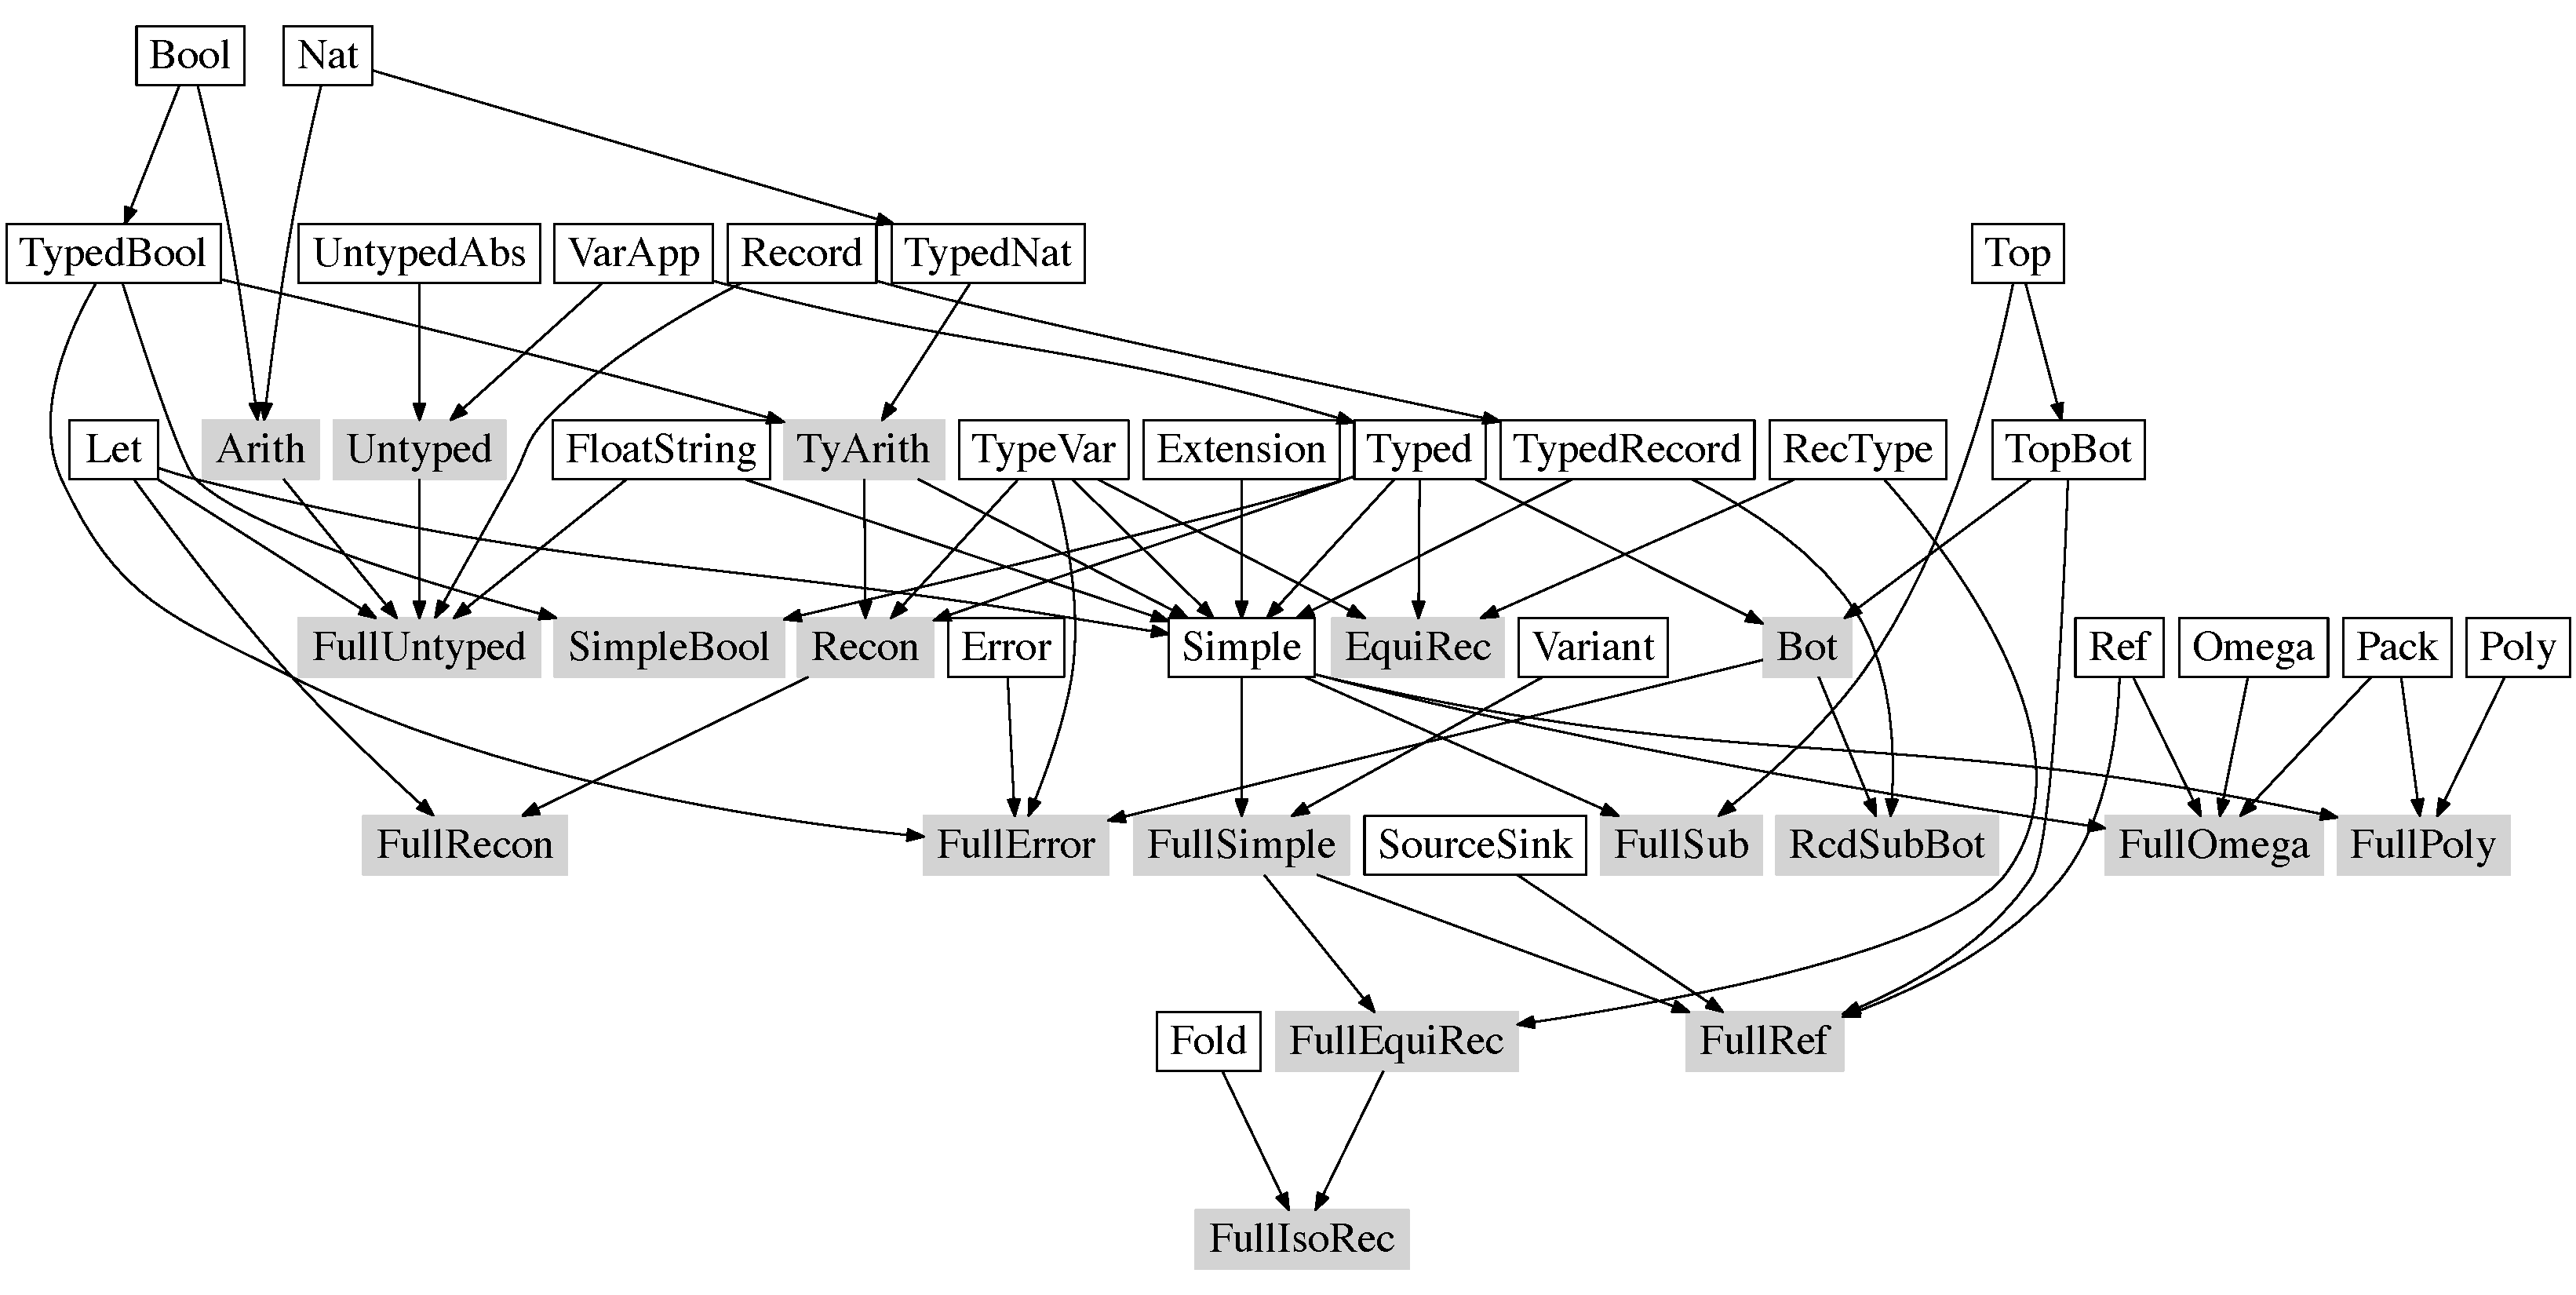
\includegraphics[width=0.8\textwidth]{resources/depGraph.pdf}
    \caption{Dependency graph of all calculi and components. Grey boxes are calculi; white boxes are components.}
    \label{fig:dependency}
\end{figure*}

Each component or language is represented by a Scala object which includes \lstinline{Alg}
for the abstract syntax, \lstinline{Print} for pretty-printing, and \lstinline{Parse} for parsing.
Since calculi and components have similar signatures, each calculus
can also be extended and reused directly. For example, calculus \lstinline{FullRef} extends from
calculus \lstinline{FullSimple}.

%% We have some naming conventions in our code, \lstinline{E} represents
%% expressions, \lstinline{T} represents types and \lstinline{K}
%% represents kinds. They are the three sorts of syntax in our case study.
%% In the component \lstinline{VarApp} we only have expressions. We use some helper traits for eliminating duplicate definitions, such as \inlinecode{EParser} containing \inlinecode{pE} for parsing expressions.

%% \lstinputlisting[linerange=9-9]{code/src/papercode/Sec6CaseStudy/Code1.scala}% APPLY:linerange=CASESTUDY_EPARSER

%% \paragraph{Composing Language Components}


%% The code of building \lstinline{Untyped} is presented in Figure~\ref{fig:casestudy-untyped}. Note that in the parser \inlinecode{Parse}, we need to override the object algebra interface and
%% parsing functions accordingly.

%% \begin{figure}[t]
%% \lstinputlisting[linerange=33-60]{code/src/papercode/Sec6CaseStudy/Code1.scala}% APPLY:linerange=CASESTUDY_UNTYPED
%% \caption{Build the \inlinecode{Untyped} calculus by composing to language components.}\label{fig:casestudy-untyped}
%% \end{figure}


%% \paragraph{Dependency Overview}

%% As shown in the graph, some components such as \lstinline{VarApp} are
%% created from scratch, while others such as \lstinline{Typed} are
%% extended from existing components.

%% From the graph, we know that common components such as \lstinline{VarApp} are reused in
%% lots of calculi. Such reuse could shorten the code considerably.
%% Next subsection examines amount of code as well as performance.

\vspace{-3pt}
\subsection{Comparison}\label{subsec:cs-comparison}

\newcommand\ourimpl{$\texttt{Mod}_{\texttt{OA}}$}
\newcommand\ilyaimpl{\texttt{NonMod}}
\newcommand\ourclass{$\texttt{Mod}_{\texttt{CLASS}}$}
\newcommand\ilyalongest{$\texttt{NonMod}_{\texttt{|||}}$}

We compared our implementation (named \ourimpl{}) with an implementation
available online\footnote{https://github.com/ilya-klyuchnikov/tapl-scala/} (named \ilyaimpl{}).
\ilyaimpl{} is suitable for comparison, because it is also
written in Scala using the same parser combinator library.
\ilyaimpl{} implements parsers 18 calculi in TAPL in a non-modular
way. Thus \ilyaimpl{} is not able to reuse existing
code when those calculi share common features.
\ourimpl{} implements the same 18 calculi, but reuse 
is possible due to modularity.

The comparison is made from two aspects. First, we want to discover
the amount of code reuse using our modular parsing approach.
For this purpose, we measured source lines of code (SLOC) of two implementations.
Second, we are interested to assess the performance penalty caused by modularity.
Thus we compared the execution time of parsing random expressions between two implementations.

\paragraph{Standard of Comparison}
In terms of SLOC, all blank lines and comments are excluded,
and we formatted the code of both implementations to ensure that
the length of each line does not exceed 120 characters. Furthermore,
because \ilyaimpl{} has extra code like semantics,
we removed all irrelevant code, only kept abstract
syntax definition, parser and pretty-printer for each calculus, to
ensure a fair comparison.

For the comparison of execution time, we built a generator to randomly
generate valid expressions for each calculus, according to its syntax. These expressions are
written to test files, one file per calculus. Each test file consists of 500
expressions randomly generated, and the size of test files varies from 20KB to 100KB.
We run the corresponding parser to parse the file and the pretty-printer to print the result.
The average execution time of 5 runs excluding reading input file was calculated, in milliseconds.

\begin{table*}\tiny
    \centering
    \resizebox{0.7\textheight}{!}{
    \begin{tabular}{|l|r|r|r|r|r|r|r|r|r|r|}
      \hline
        \multirow{2}{*}{\bfseries Calculus Name} & \multicolumn{3}{ c| }{\bfseries SLOC} & \multicolumn{7}{ c| }{\bfseries Time (ms)} \\ \cline{2-11}
        \multicolumn{1}{|c|}{} & \ilyaimpl{} & \ourimpl{} & \bfseries (+/-)\% & \ilyaimpl{} & \ourimpl{} & \bfseries (+/-)\% & \ilyalongest{} & \bfseries (+/-)\% & \ourclass{} & \bfseries (+/-)\% \\
      \hline
      \begin{tabular}{|c|c|c|}
  \hline
  t1 & t2 & t3 \\
  y1 & val1 & val4 \\
  y2 & val2 & val3 \\
  \hline
\end{tabular}

      \hline
      \multicolumn{7}{c}{}
    \end{tabular}}
 	\vspace{-5pt}
    \caption{Comparison of SLOC and execution time.}
    \label{tab:comparison}
    \vspace{-0.3cm}
\end{table*}

\vspace{-4pt}
\paragraph{Comparison Results}
Table \ref{tab:comparison} shows results of the comparison.
Let us only check \ourimpl{} and \ilyaimpl{} for now.
The overall result is that 69.2\% of code is reduced using our
approach, and our implementation is 42.7\% slower.

The good SLOC result is because of that the code of common language features
are reused many times in the whole case study. We can see that in the first two calculi
\lstinline{Arith} and \lstinline{Untyped} we are not better than \ilyaimpl{},
because in such two cases we do not reuse anything.
However in the following 16 calculi, we indeed reuse language components.
In particular, the calculi \inlinecode{EquiRec} and some others are only 22 lines
in our implementation, because we only compose existing code.

To discover the reasons of slower execution time, we made experiments
on two possible factors, which are Object Algebras and the longest match alternative combinator.
We use Object Algebras for ASTs and the longest match alternative combinator \inlinecode{|||} for parsing,
while \ilyaimpl{} uses case class and the ordinary alternative combinator.
Therefore, we implemented two more versions. One is a modified version of our implementation,
named \ourclass{}, with Object Algebras replaced by case class for the ASTs.
The other is a modified version of \ilyaimpl{}, named \ilyalongest{},
using the longest match alternative combinator instead of the ordinary one.

%% \begin{table*}
%%     \centering
%%     \begin{tabular}{|l|r|r|r|r|r|r|r|}
%%       \hline
%%         \multirow{2}{*}{\bfseries Calculus Name} & \ilyaimpl{} & \multicolumn{2}{ c| }{\ourimpl{}} & \multicolumn{2}{ c| }{\ilyalongest{}} & \multicolumn{2}{ c| }{\ourclass{}} \\ \cline{2-8}
%%         \multicolumn{1}{|c|}{} & \multicolumn{1}{c|}{\bfseries Time} & \bfseries Time & \bfseries (+/-)\% & \bfseries Time & \bfseries (+/-)\% & \bfseries Time & \bfseries (+/-)\% \\
%%       \hline
%%         Arith & 741 & 913 & +23.2 & 793 & +7.0 & 932 & +25.8 \\
%%         Untyped & 770 & 1018 & +32.2 & 821 & +6.6 & 1007 & +30.8 \\
%%         FullUntyped & 1297 & 1854 & +42.9 & 1343 & +3.5 & 1767 & +36.2 \\
%%         TyArith & 746 & 888 & +19.0 & 772 & +3.5 & 918 & +23.1 \\
%%         SimpleBool & 1376 & 1782 & +29.5 & 1494 & +8.6 & 1824 & +32.6 \\
%%         FullSimple & 1441 & 2270 & +57.5 & 1574 & +9.2 & 2226 & +54.5 \\
%%         Bot & 1080 & 1287 & +19.2 & 1078 & -0.2 & 1306 & +20.9 \\
%%       %\hline
%%         %\multicolumn{1}{|c|}{\dots} & \multicolumn{7}{c|}{\dots} \\
%%       %\hline
%%         FullRef & 1438 & 2291 & +59.3 & 1544 & +7.4 & 2142 & +49.0 \\
%%         FullError & 1410 & 1946 & +38.0 & 1524 & +8.1 & 1981 & +40.5 \\
%%         RcdSubBot & 1247 & 1524 & +22.2 & 1285 & +3.0 & 1612 & +29.3 \\
%%         FullSub & 1320 & 1979 & +49.9 & 1393 & +5.5 & 1899 & +43.9 \\
%%         FullEquiRec & 1407 & 2200 & +56.4 & 1561 & +10.9 & 2156 & +53.2 \\
%%         FullIsoRec & 1492 & 2253 & +51.0 & 1648 & +10.5 & 2236 & +49.9 \\
%%         EquiRec & 994 & 1254 & +26.2 & 1048 & +5.4 & 1304 & +31.2 \\
%%         Recon & 1044 & 1482 & +42.0 & 1128 & +8.0 & 1506 & +44.3 \\
%%         FullRecon & 1094 & 1645 & +50.4 & 1161 & +6.1 & 1652 & +51.0 \\
%%         FullPoly & 1398 & 2086 & +49.2 & 1511 & +8.1 & 2019 & +44.4 \\
%%         FullOmega & 1451 & 2352 & +62.1 & 1582 & +9.0 & 2308 & +59.1 \\
%%       \hline
%%         Total & 21746 & 31024 & +42.7 & 23260 & +7.0 & 30795 & +41.6 \\
%%       \hline
%%         \multicolumn{8}{c}{}
%%     \end{tabular}
%%     \caption{Execution time of four implementations.}
%%     \label{tab:ext-comparison}
%% \end{table*}

The right part of Table \ref{tab:comparison} suggests that the difference of running time between
using Object Algebras and class is little, roughly 1\%.
The use of longest match combinator slows the performance by 7\%. The main reason of slower
execution time may be the overall structure of the modular parsing approach, because we indeed have
more intermediate function calls and method overriding. However, it is worth mentioning that
because of the memoization technique of Packrat parsers, we are only constant times
slower, the algorithmic complexity is still the same.
Since the slowdown seems to be caused by extra method
dispatching, in future work we wish to investigate techniques like
partial evaluation or meta-programming to eliminate such cost. The
work by B{\'e}guet and Manohar~\cite{Beguet:2014} is an interesting starting point.


\section{Related Work}\label{sec:relatedwork}

%- extensible parsing, language workbenches: rats, noa (this one already uses OA), modular semantic actions, (syntactic modularity, no separate compilation, modular type-checking)
%(read more papers, see if they talk about this issue, some potential solutions)
%(attribute grammars?)
%
%- parser combinators for type-checking, previous work has not shown how to support modularity (ASTs); left-recursion and back-tracking in related techniques
%
%- modularity: object algebras, dtc and mrm (problem with parsing, is there any related work? (PB: a paper on unfolds: build the AST))
%
%(parsing in Javascript: using delegation, does it support modular AST)
%
%noa, shy: shy: only override some interesting cases (transformation is tedious)
%bruijn indices: parsing + transformation

Our work touches upon several topics including extensible parsing,
parser combinators and extensibility techniques. However, as far as we
know there's no work that discusses how to do statically type-safe and
separately compilable modular parsing.

\begin{comment}
There has been a
great amount of related papers on those topics. Some
inspired us of this paper and encourage us for more exploration. This
section will try to lead a discussion on what difference we have made.
\end{comment}

\paragraph{Syntactically Extensible Parsing}
Extensible parser generators~\cite{antlr1995,Grimm2006,Gouseti2014,Warth2016}
are a mainstream area of modular syntax and parsing. They allow users to write
modular grammars, where new
non-terminals and production rules can be introduced, some can even
override existing rules in the old grammar modules. For instance,
\textit{Rats!}~\cite{Grimm2006} constructs its own module system for
the collection of grammars, while NOA~\cite{Gouseti2014} uses Java
annotation to collect all information before producing an ANTLR~\cite{antlr1995} grammar
and the parsing code. Those parser
generators focus on the \textit{syntactic extensibility} of grammars:
they rely on whole compilation to generate a global parser, even if
there is only a slight modification in the grammar. Some of those
parser generators may statically check the correctness and unambiguity
of grammars. In contrast, because our approach is based on parser
combinators, there is no support for ambiguity checking.  However, as
far as we are aware, no extensible parser generators support separate
compilation or modular type-checking.

Macro systems like the C preprocessor, C++ templates and
Racket~\cite{Tobin-Hochstadt2011}, and other meta-programming
techniques are a similar area aiming at syntactic extensibility.
SugarJ~\cite{Erdweg2011} conveniently introduces syntactic sugar for
Java using library imports. Composition of syntactic sugar is easy for
users, but it requires many rounds of parsing and adaption, hence
significantly affects the efficiency of compilation. Since the
implementation was based on SDF~\cite{Heering1989} and
Stratego~\cite{Visser2001}, it does not support separate
compilation. Racket adopts a macro system for library-based language
extensibility~\cite{Tobin-Hochstadt2011}. It uses
attributed ASTs for contextual
information, and extensions can be integrated in a modular
way. However such modularity is not flexible enough for language
unification, as the syntax is only built from extensions.
%Moreover,
%existing macros cannot be further changed after
%definition. \haoyuan{correct?}
Extensible
compilers like JastAdd~\cite{Ekman2007} and
Polyglot~\cite{Nystrom2003} also support extensible parsing, but this
is mostly done using parser generators. They focus on the
extensions to a host language. Those techniques are short of type safety in a modular
setting as well.

%\bruno{Have you read
%Languages as Libraries? That is probably an important reference, which
%I think we should cite.}
%\haoyuan{what about
%  metafront? it is a macro system but does it have type safety?}
%\haoyuan{Extensible syntax with lexical scoping?} \haoyuan{"Extensible
%  syntax" proposes a system for extensible syntax, where users write
%  EDSLs in their language with concrete syntax. Users can write rules
%  for type-based disambiguation. But separate compilation is again not
%  mentioned. Shall we mention that thesis?} \haoyuan{attribute
%  grammars?}

\paragraph{Extensible Parsing Algorithm}
\textit{Parse table composition}~\cite{bravenboer2008parse}
is an approach where grammars are compiled to
modular parse tables. Those parse tables are expressed as DFAs
or NFAs, and later they can be composed by an algorithm, to provide
separate compilation for parsing. The generation of parse tables can
be quite expensive in terms of performance. The approach
is quite different from ours, since it uses parse
 tables, whereas we use parser combinators.
Our approach supports both
\emph{separate compilation} as well as \emph{modular
  type-checking}. Moreover, the extensibility of parsing is further
available at language composition and lexical level.

%\haoyuan{we do not have explicit
%  correspondence/relationship between abstract syntax and the parser.}

\paragraph{Parser Combinators} Parser combinators have become more and more
popular since~\cite{burge1975,Wadler1985}. Many parsing libraries produce recursive descent
parsers by introducing functional monadic
parser combinators~\cite{nott237}. Parsec~\cite{Leijen2001} is
perhaps the most popular parser combinator library in this line.
It is widely used in Haskell (with various ``clones'' in other languages)
for context-sensitive grammars with infinite lookahead. Nevertheless,
Parsec users suffer from manual left-recursion elimination,
high cost for backtracking and longest match composition issues,
as we discussed in Section~\ref{subsec:challenges}. Those limitations make Parsec
(and similar parsing techniques) inadequate for modular parsing.

Some more recent work on parser
combinators~\cite{Ford2002,Might2011,Frost2008} proposed a series of
novel parsing techniques that address the issue of
left-recursion. We have selected Packrat parsing due to its simplicity in Scala,
but in general it can also have alternatives.

\paragraph{Extensibility} Various design patterns~\cite{gamma1995design} in multiple
languages, have been proposed over the years to address extensibility
problems, such as the Expression Problem~\cite{wadler1998expression}.
The famous ``Datatypes \`a
la Carte'' (DTC)~\cite{swierstra2008data} approach represents modular ASTs using co-products
of every two functors. Several variants of DTC have been later proposed~\cite{Bahr2011,Bahr2014,Oliveira2015}.
All of that work essentially covers how to traverse and
consume extensible ASTs. However they do not
address the problem of \emph{modularly
parsing extensible ASTs}. Only in Bahr's~\cite{Bahr2011} work \emph{unfolds} is briefly mentioned,
yet it does not cover parsing.

There are also many design patterns in OO languages that achieve
type-safe extensibility~\cite{torgersen2004expression,odersky2005independently,oliveira2009modular,Oliveira:2012,wang2016expression}. We chose Object Algebras~\cite{Oliveira:2012} because the pattern is
relatively lightweight and makes good use of existing OO features,
such as inheritance, generics and subtyping. As seen throughout the paper,
the parsing code is concise and expressive using Object Algebras.
On the other hand we are unware of any work on OOP
that has covered how to do modular parsing for extensible ASTs.

It is worth mentioning that Scala case classes~\cite{emir2007matching} provide a near
solution to the Expression Problem. Case classes can be
modularly added, but they do not enforce
exhaustiveness of pattern matching for extensible operations. In other
words run-time pattern matching errors can happen when writing extensible code with case classes. So that full static type-safety is not ensured. Nevertheless case classes are a pragmatic approach, which is
widely used in practice. Therefore, modular parsing techniques may be
of value for extensible code using case classes.  The approach we
presented in Section~\ref{sec:inheritance} can readily be adapted to case classes:
all that the users need to do is to use case classes, instead of
standard OO classes in their code.

\begin{comment}
Moreover, in~\cite{Oliveira:2012} the authors have discussed the
composition of algebras. In our parsing approach, a parser consumes an
algebra, which is delegated to return the results, during its process
of parsing. Having a set of algebras, it requires multiple parsing
with several times of invocation, which leads to redundant work.
Instead, algebras are supposed to be composed into one before the
invocation of the parser. Bahr et al. lead a similar discussion
in~\cite{Bahr2011}, where queries (or \textit{catamorphisms}) and
transformations (or \textit{homomorphisms}) are composable. They have
also mentioned the dual process of folds, namely
\textit{anamorphisms}. It is potentially related to our work, as
parsing is a representative kind of unfolds, whereas they only
discussed the composition of a cv-coalgebra and a term homomorphism,
which differs from modular parsing.
\end{comment}

\begin{comment}
Another interesting observation from Section~\ref{sec:algebrasandparsing}, is that parsers with
Object Algebras generate ``implicit objects'', which are actually functions of
type \lstinline{Alg[E]} \lstinline{=>} \lstinline{E} for generic \lstinline{E}.
Patterns of operations on such functions are captured by the original paper~\cite{Oliveira:2012}, called
\textit{queries} and \textit{transformations}, together with the composition of algebras.
They are quite useful, for instance, we have two operations (like the aforementioned \lstinline{Print} and \lstinline{Eval}) to be fed to the parser. If we feed them separately, it is tedious to parse the same input twice. Instead we can compose them in advance before the feeding. On the other hand, one would think this pattern is too limited to use against objects that traditional parsers generate. For example, there are a lot of transformations (or desugarings) on intermediate ASTs in the design of a compiler. Transformation algebras are helpful in that case. They can even be composed in a linear pipeline-style before a query algebra is delegated. The Shy framework~\cite{Zhang2015} has captured those patterns, and it generates templates for them, so that users only need to override a few interesting cases, conveniently. The idea of overriding existing cases was also
proposed in MRM~\cite{Oliveira2015}. They are potentially useful to our approach. Regarding overriding, our approach allows existing parsing code to be overridden during inheritance.
\end{comment}


\section{Conclusion}\label{sec:conclusion}

This paper presents a solution for semantically modular parsing. It not only
enables parsers to evolve with the syntax together, but also allows them to be modularly type-checked and separately compiled.

Based on parser combinators, we identify the the algorithmic challenges of building modular parsers, and show that Packrat parsing is suitable as the underlying parsing technique. Our solution does not require advanced language features. We show that with standard OO techniques including inheritance and overriding, it is practicable to build modular parsers for OO ASTs. However, the extensibility issue of traditional OO ASTs motivates us to adopt Object Algebras for full extensibility and more useful features.

Abstracting language features as reuseable components can be achieved based on our solution, which is useful for rapid language prototyping. Our solution does not rely on particular techniques. On the contrary, it is a general framework customizable by the user. The TAPL case study shows that we can obtain considerable code reuse (69\%) than a non-modular implementation, using our modular parsing approach and language feature abstraction.

There are certainly some aspects can be improved. We observed that the glue code of composition appears to be boilerplate. Such an issue refers to family polymorphism, and we could solve it by language features or meta-programming techniques. Moreover, we can possibly adopt the Shy framework~\cite{Zhang2015} and algebra composition patterns~\cite{oliveira2013feature}, to improve the usage of Object Algebras.

For future work, we will experiment more on how open recursion contributes to extensible parsing in functional languages, by making use of laziness. It is also interesting to see that parsing, to some extent, can be viewed as a special example of \textit{unfolds}. So it is worthwhile considering to generalize our approach under certain circumstances.


%===============================================================================

\bibliographystyle{plain}
\bibliography{paper}

\appendix

\end{document}

%%% Local Variables:
%%% mode: latex
%%% TeX-master: "."
%%% End:
